\documentclass{article}
\usepackage{pgfplots}
 \pgfplotsset{compat=newest}

 \begin{document}

Introduction

In recent years the push for and the growth of Large Language Models (LLM) provided new challenges for processor and compiler developers to improve the throughput and performance of such models. The main challenge is to stay within the constraints of already existing hardware. Although hardware accelerators entering the market in relative rapid succession, companies may not be willing to upgrade their compute ressources with each new generation of processors and accelerators. Usually a software upgrade and tool upgrade is much more common and easier to achieve compared to an actual hardware upgrade.  
Essentially there are two areas, which are targeted to improve performance of LLMs. First there is the improvement of the hardware by utilizing new hardware architectures and improving existing hardware architectures by adding specific features, which benefit the processing of neural network workloads. The other area is the improvement by software tools. Specifically AI compilers are under development, which boost the performance of exising hardware by utilizing the specific AI accelerating features, an also need to adapt quickly to support new features of new hardware. These optimizations are often in the area of parallel execution of workloads, faster data transfer between nodes and faster loading of kernels into the hardware to name a few. 
One newer optimization technique is the fusion of multiple neural network nodes into one single node. This paper discusses fusion of a avgpool operation with a gelu operation. The following sections provide a brief discussion of the underlying idea, then discuss some of the implementation and test features and environment. Lastly measured results are presented and a conclusion is given. 

Motivation 

A neural network workload constitutes of many nodes which mostly are executed individually or in eager mode. This means even with accelerating hardware, each node is executed on an individual basis and therefore the data is loaded in and out of the accelerator after each operation. A huge amount of data may be loaded to the accelerator, which then in a very aggressive highly parallel effort, performs such an operation quickly utilizing the parallel feature of the hardware accelerator and then load the result of said operation back to the host processor. A second node is processed in the exact same way, which means that the same or maybe a reduced or enlarged amount of data is loaded into the accelerator and the appropriate process is performed again. The neverthless means that data which might as well be processed within the same hardware is uploaded and downloaded between processing steps albeit being already at the correct location or stored in the correct memory.  
By fusing nodes the additional upload and download step of interim results are removed and the appropriate steps are directly performed. This usually leads to a considerable improvement in throughput and performance of the exact same model. We can see this specifically in the combination of matrix multiplication with immediately following activation functions. The optimization of matrix multiplication and its fusion with activation functions seems to be already widely discussed[]. What is also mentioned in many publications is the overall impact on existing models, whereas there is little to no discussion about the impact of the individual contributing node, which would be an utmost important tool for developers of original neural network architectures. In this paper we discuss one specific combination of operations, which are very common in the context of Large Language Models. The first is the avgPool2D function and the second is the gelu function. Other publications will follow to discuss other combinations of operations. 

The approach
Different solutions were executed to compare the runtime of a avgpool operation and a gelu operation between CPU and CUDA solutions. A small model with one avgPool2D operation and one gelu operation with flexible shapes is implemented in C++ to run on a CPU. Then a total of three kernels are developed in CUDA. The first kernel represents the avgPool2d operation, the second kernel represents the Gelu operation and the third kernel represents the fused kernel, which constitutes of the said avgPool2D operation and the gelu operation but it is implemented as one kernel only. 

The implementation of the avgPool2D kernel is based on the following mathematical representation:
 

\(avgPool2D(N_i, C_j, h, w)  = \frac{1}{kH * kW} \sum_{m=0}^{kH-1} \sum_{n=0}^{kW-1}
                               input(N_i, C_j, stride[0] \times h + m, stride[1] \times w + n)\)


The gelu kernel is based on the following mathematical definition:  

\( GELU(x) = 0.5 * x * (1 + \tanh(\sqrt{2 / \pi} * (x + 0.044715 * x^3)))\)

We recognize that there are proposals to improve the gelu operation considerably by using partial functions which include linear optimizations. 


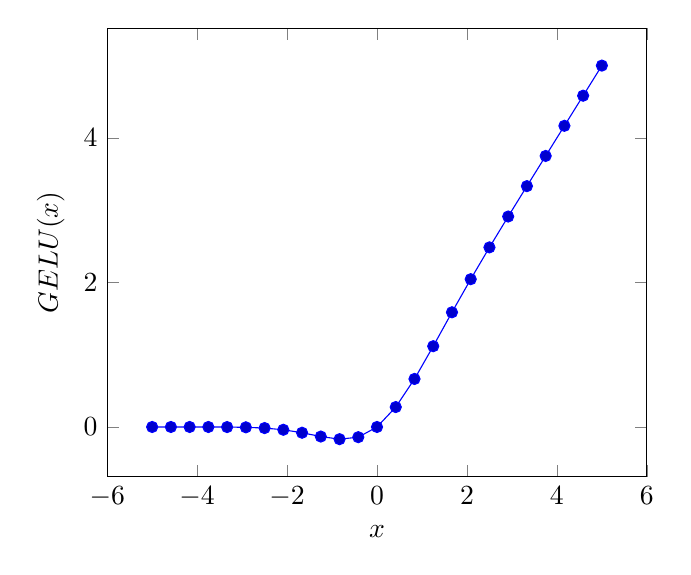
\begin{tikzpicture}

  \begin{axis}[ 
    xlabel=$x$,
    ylabel={$GELU(x)$}
  ] 
    \addplot {0.5 * x * (1 + tanh(sqrt(2/pi) * (x +0.044715 * x*x*x))) }; 
  \end{axis}

\end{tikzpicture}


In the following we shows the results when running the individual kernels on CPU, then we show the combined solution running on CPU. Further we show the performance of the two CUDA kernels running back to back on a CUDA platform, and finally compare that with the fused kernel solution, which shows the real benefit of performing fusion in the first place. 

Results

The first result is based on a CPU implementation of avgPool2D in C++ on a PC. In fig... we can clearly identify a linear behaviour based on the number of input elements. The kernel size as well as the stride size are set to (8x8)  


\begin{tikzpicture}
\begin{axis}[
    title=avgpool on CPU,
    xlabel={$dx$},
    ylabel={$sec$},
    legend entries={$dy=512$,$dy=1024$,$dy=1536$,$dy=2048$,$dy=2560$, $dy=3072$},
    legend pos=north west,
]
    \addplot [red] table {cpu_avgPool_dimi_512.dat};
    \addplot [blue] table {cpu_avgPool_dimi_1024.dat};
    \addplot [green] table {cpu_avgPool_dimi_1536.dat};
    \addplot [orange] table {cpu_avgPool_dimi_2048.dat};
    \addplot [magenta] table {cpu_avgPool_dimi_2560.dat};
    \addplot [yellow] table {cpu_avgPool_dimi_3072.dat};

\end{axis}
\end{tikzpicture}

The next result is showing the complete result with Gelu. The addition of Gelu hardly contributes to the 


\begin{tikzpicture}
\begin{axis}[
    title=avgpool with gelu on CPU,
    xlabel={$dx$},
    ylabel={$sec$},
    legend entries={$dy=512$,$dy=1024$,$dy=1536$,$dy=2048$,$dy=2560$, $dy=3072$},
    legend pos=north west,
]
    \addplot [red] table {cpu_avgPoolGelu_dimi_512.dat};
    \addplot [blue] table {cpu_avgPoolGelu_dimi_1024.dat};
    \addplot [green] table {cpu_avgPoolGelu_dimi_1536.dat};
    \addplot [orange] table {cpu_avgPoolGelu_dimi_2048.dat};
    \addplot [magenta] table {cpu_avgPoolGelu_dimi_2560.dat};
    \addplot [yellow] table {cpu_avgPoolGelu_dimi_3072.dat};

\end{axis}
\end{tikzpicture}

The following example shows that exercising Gelu on a CPU does not significantly change the overall runtime. The main explanation is that there is no additional allocation of memory involved since Gelu directly writes back to the same element. Further the number of elements is reduced now by 64, because the avgPool2D operation uses a 8x8 inner dimensions for our example.

\begin{tikzpicture}
\begin{axis}[
    title=avgpool with and without gelu on CPU,
    xlabel={$dx$},
    ylabel={$sec$},
    legend entries={$only avgpool$, $with gelu$},
    legend pos=north west,
]
    \addplot [red] table {cpu_avgPool_dimi_3072.dat};
    \addplot [blue] table {cpu_avgPoolGelu_dimi_3072.dat};

\end{axis}
\end{tikzpicture}

 

Now the CUDA results are presented. The first results are based on the avgPool2D cuda kernel. It shows that the parallel execution leads to almost no difference between smaller and larger workloads. The presented workloads are still small and therefore the major impact comes from the overhead of engaging with the GPU in the first place. Nevertheless the results clearly show that the CUDA implementation has a huge impact on the performance. 

\begin{tikzpicture}
\begin{axis}[
    title=avgpool on CUDA,
    xlabel={$dx$},
    ylabel={$sec$},
    legend entries={$dy=512$,$dy=1024$,$dy=1536$,$dy=2048$,$dy=2560$, $dy=3072$},
    legend pos=north east,
]
    \addplot [red] table {cuda_avgPool_dimi_512.dat};
    \addplot [blue] table {cuda_avgPool_dimi_1024.dat};
    \addplot [green] table {cuda_avgPool_dimi_1536.dat};
    \addplot [orange] table {cuda_avgPool_dimi_2048.dat};
    \addplot [magenta] table {cuda_avgPool_dimi_2560.dat};
    \addplot [yellow] table {cuda_avgPool_dimi_3072.dat};

\end{axis}
\end{tikzpicture}



If we only engage the Gelu kernel it seems that for most cases the overhead to engage with the GPU has a higher impact than performing the Gelu directly on the CPU. Nevertheless part of it is misleading since on the CPU we do not count the impact of the memory allocation, which is already done as part of the avgPool2D output matrix memory allocation. 


\begin{tikzpicture}
\begin{axis}[
    title=gelu on CUDA,
    xlabel={$dx$},
    ylabel={$sec$},
    legend entries={$dy=512$,$dy=1024$,$dy=1536$,$dy=2048$,$dy=2560$, $dy=3072$},
    legend pos=north east,
]
    \addplot [red] table {cuda_Gelu_dimi_512.dat};
    \addplot [blue] table {cuda_Gelu_dimi_1024.dat};
    \addplot [green] table {cuda_Gelu_dimi_1536.dat};
    \addplot [orange] table {cuda_Gelu_dimi_2048.dat};
    \addplot [magenta] table {cuda_Gelu_dimi_2560.dat};
    \addplot [yellow] table {cuda_Gelu_dimi_3072.dat};

\end{axis}
\end{tikzpicture}


To provide some better datapoints the next plot shows running the avgPool2D and the Gelu running back to back, yet using separate kernels. We can clearly also see that there is some overhead compared to the prior solution. 

\begin{tikzpicture}
\begin{axis}[
    title=avgPool and gelu sequential CUDA,
    xlabel={$dx$},
    ylabel={$sec$},
    legend entries={$dy=512$,$dy=1024$,$dy=1536$,$dy=2048$,$dy=2560$, $dy=3072$},
    legend pos=north east,
]
    \addplot [red] table {cuda_avgPoolGelu_notMerged_512.dat};
    \addplot [blue] table {cuda_avgPoolGelu_notMerged_1024.dat};
    \addplot [green] table {cuda_avgPoolGelu_notMerged_1536.dat};
    \addplot [orange] table {cuda_avgPoolGelu_notMerged_2048.dat};
    \addplot [magenta] table {cuda_avgPoolGelu_notMerged_2560.dat};
    \addplot [yellow] table {cuda_avgPoolGelu_notMerged_3072.dat};

\end{axis}
\end{tikzpicture}

The best result is achieved by using the fused kernel. The fused kernel incorporates avgPool2D and Gelu in one kernel and therefore the output of the avgPool2D is directly processed. The first result does not need to be copied to the main mamory and back to the kernel memory of the Gelu kernel any more. This allows to shave off a significant portion of the runtime and improve the performance significantly. 


\begin{tikzpicture}
\begin{axis}[
    title=avgPool and gelu fused CUDA,
    xlabel={$dx$},
    ylabel={$sec$},
    legend entries={$dy=512$,$dy=1024$,$dy=1536$,$dy=2048$,$dy=2560$, $dy=3072$},
    legend pos=north east,
]
    \addplot [red] table {cuda_avgPoolGelu_merged_512.dat};
    \addplot [blue] table {cuda_avgPoolGelu_merged_1024.dat};
    \addplot [green] table {cuda_avgPoolGelu_merged_1536.dat};
    \addplot [orange] table {cuda_avgPoolGelu_merged_2048.dat};
    \addplot [magenta] table {cuda_avgPoolGelu_merged_2560.dat};
    \addplot [yellow] table {cuda_avgPoolGelu_merged_3072.dat};

\end{axis}
\end{tikzpicture}

Conclusion

We conclude that kernel fusion has a significant impact on the performance and the throuput of a model. Although the fused kernel was not integrated into a realistic LLM workload this initial research already shows significant progress. The final figure combines the most significant results. We can see that only when a small matrix is used, i.e. at or below 128x3096, the CPU solution may be faster. 

\begin{tikzpicture}
\begin{axis}[
    title=CPU vs CUDA vs fused CUDA,
    xlabel={$dx$},
    ylabel={$sec$},
    legend entries={$CPU$, $CUDA$,$CUDA fused$},
    legend pos=north west,
]
    \addplot [red] table {cpu_avgPoolGelu_dimi_3072.dat};
    \addplot [blue] table {cuda_avgPoolGelu_notMerged_3072.dat};
    \addplot [green] table {cuda_avgPoolGelu_merged_3072.dat};

\end{axis}
\end{tikzpicture}


The herein presented results are based on the implementation of a new CUDA based library, which concentrates solely on fused kernels for AI workloads. 

[] https://arxiv.org/abs/2108.13342
[] https://dl.acm.org/doi/10.1145/3520142



\end{document}